%% Manuscript for Computational Statistics (Springer).
%% Compile with the Springer Nature LaTeX template (sn-jnl.cls), e.g. in the
%% Overleaf "Springer Nature LaTeX Template" project: upload this file, refs.bib,
%% numbers.tex, tables/ and figures/ (no subfolders are required by the journal:
%% see README_SUBMISSION_TR.md for flattening). Numbers come from numbers.tex and
%% tables/*.tex, which are generated by analysis/make_tables.py.

\documentclass[pdflatex,sn-mathphys-ay]{sn-jnl}

\usepackage{graphicx}
\usepackage{multirow}
\usepackage{amsmath,amssymb,amsfonts}
\usepackage{amsthm}
\usepackage{booktabs}
\usepackage{xcolor}
\usepackage{textcomp}

\theoremstyle{thmstyleone}
\newtheorem{proposition}{Proposition}
\theoremstyle{thmstylethree}
\newtheorem{remark}{Remark}

\raggedbottom

% Generated by analysis/make_tables.py from analysis/out; do not edit by hand.
\newcommand{\NDecisions}{120}
\newcommand{\NBoot}{2,000}
\newcommand{\NRecompute}{2,100}
\newcommand{\RecomputeMaxDiff}{\ensuremath{2.2\times 10^{-16}}}
\newcommand{\BalQwk}{0.62}
\newcommand{\RegEndQwk}{0.44}
\newcommand{\RegQwkQwk}{0.10}
\newcommand{\RegMaeQwk}{0.43}
\newcommand{\RegMmaeQwk}{0.34}
\newcommand{\RankEndQwk}{3.95}
\newcommand{\RankQwkQwk}{2.38}
\newcommand{\AgrQwkQwk}{1.00}
\newcommand{\AgrQwkMae}{0.36}
\newcommand{\AgrQwkAmae}{0.41}
\newcommand{\AgrQwkMmae}{0.37}
\newcommand{\AgrQwkMfone}{0.63}
\newcommand{\AgrQwkRps}{0.26}
\newcommand{\AgrQwkCon}{0.71}
\newcommand{\BalMae}{0.04}
\newcommand{\RegEndMae}{0.70}
\newcommand{\RegQwkMae}{0.49}
\newcommand{\RegMaeMae}{0.04}
\newcommand{\RegMmaeMae}{0.84}
\newcommand{\RankEndMae}{5.03}
\newcommand{\RankQwkMae}{4.47}
\newcommand{\AgrMaeQwk}{0.36}
\newcommand{\AgrMaeMae}{1.00}
\newcommand{\AgrMaeAmae}{0.12}
\newcommand{\AgrMaeMmae}{0.03}
\newcommand{\AgrMaeMfone}{0.24}
\newcommand{\AgrMaeRps}{0.68}
\newcommand{\AgrMaeCon}{0.22}
\newcommand{\BalAmae}{0.81}
\newcommand{\RegEndAmae}{0.50}
\newcommand{\RegQwkAmae}{0.47}
\newcommand{\RegMaeAmae}{0.70}
\newcommand{\RegMmaeAmae}{0.29}
\newcommand{\RankEndAmae}{4.12}
\newcommand{\RankQwkAmae}{4.45}
\newcommand{\AgrAmaeQwk}{0.41}
\newcommand{\AgrAmaeMae}{0.12}
\newcommand{\AgrAmaeAmae}{1.00}
\newcommand{\AgrAmaeMmae}{0.56}
\newcommand{\AgrAmaeMfone}{0.47}
\newcommand{\AgrAmaeRps}{0.08}
\newcommand{\AgrAmaeCon}{0.44}
\newcommand{\BalMmae}{0.96}
\newcommand{\RegEndMmae}{0.33}
\newcommand{\RegQwkMmae}{0.43}
\newcommand{\RegMaeMmae}{0.78}
\newcommand{\RegMmaeMmae}{0.04}
\newcommand{\RankEndMmae}{3.02}
\newcommand{\RankQwkMmae}{4.88}
\newcommand{\AgrMmaeQwk}{0.37}
\newcommand{\AgrMmaeMae}{0.03}
\newcommand{\AgrMmaeAmae}{0.56}
\newcommand{\AgrMmaeMmae}{1.00}
\newcommand{\AgrMmaeMfone}{0.37}
\newcommand{\AgrMmaeRps}{0.01}
\newcommand{\AgrMmaeCon}{0.51}
\newcommand{\BalMfone}{0.72}
\newcommand{\RegEndMfone}{0.45}
\newcommand{\RegQwkMfone}{0.26}
\newcommand{\RegMaeMfone}{0.52}
\newcommand{\RegMmaeMfone}{0.25}
\newcommand{\RankEndMfone}{3.98}
\newcommand{\RankQwkMfone}{3.73}
\newcommand{\AgrMfoneQwk}{0.63}
\newcommand{\AgrMfoneMae}{0.24}
\newcommand{\AgrMfoneAmae}{0.47}
\newcommand{\AgrMfoneMmae}{0.37}
\newcommand{\AgrMfoneMfone}{1.00}
\newcommand{\AgrMfoneRps}{0.15}
\newcommand{\AgrMfoneCon}{0.41}
\newcommand{\BalRps}{0.00}
\newcommand{\RegEndRps}{0.67}
\newcommand{\RegQwkRps}{0.53}
\newcommand{\RegMaeRps}{0.04}
\newcommand{\RegMmaeRps}{0.88}
\newcommand{\RankEndRps}{5.15}
\newcommand{\RankQwkRps}{4.58}
\newcommand{\AgrRpsQwk}{0.26}
\newcommand{\AgrRpsMae}{0.68}
\newcommand{\AgrRpsAmae}{0.08}
\newcommand{\AgrRpsMmae}{0.01}
\newcommand{\AgrRpsMfone}{0.15}
\newcommand{\AgrRpsRps}{1.00}
\newcommand{\AgrRpsCon}{0.14}
\newcommand{\BalCon}{0.78}
\newcommand{\RegEndCon}{0.24}
\newcommand{\RegQwkCon}{0.29}
\newcommand{\RegMaeCon}{0.66}
\newcommand{\RegMmaeCon}{0.21}
\newcommand{\RankEndCon}{2.75}
\newcommand{\RankQwkCon}{3.52}
\newcommand{\AgrConQwk}{0.71}
\newcommand{\AgrConMae}{0.22}
\newcommand{\AgrConAmae}{0.44}
\newcommand{\AgrConMmae}{0.51}
\newcommand{\AgrConMfone}{0.41}
\newcommand{\AgrConRps}{0.14}
\newcommand{\AgrConCon}{1.00}
\newcommand{\RegOwnMax}{0.13}
\newcommand{\FriedEndChi}{22.7}
\newcommand{\FriedEndP}{\ensuremath{<}0.001}
\newcommand{\FriedQwkChi}{20.2}
\newcommand{\FriedQwkP}{\ensuremath{=}0.003}
\newcommand{\NemenyiCD}{2.01}
\newcommand{\WilPAmae}{0.611}
\newcommand{\WilPosAmae}{7}
\newcommand{\WilNegAmae}{10}
\newcommand{\WilMedAmae}{\ensuremath{-}0.003}
\newcommand{\WilMeanAmae}{\ensuremath{-}0.022}
\newcommand{\QwkCostMedAmae}{\ensuremath{-}0.015}
\newcommand{\QwkCostNegAmae}{14}
\newcommand{\QwkCostPAmae}{0.002}
\newcommand{\WilPMfone}{0.847}
\newcommand{\WilPosMfone}{8}
\newcommand{\WilNegMfone}{7}
\newcommand{\WilMedMfone}{0.000}
\newcommand{\WilMeanMfone}{\ensuremath{-}0.003}
\newcommand{\QwkCostMedMfone}{\ensuremath{-}0.003}
\newcommand{\QwkCostNegMfone}{14}
\newcommand{\QwkCostPMfone}{0.003}
\newcommand{\WilPCon}{0.008}
\newcommand{\WilPosCon}{8}
\newcommand{\WilNegCon}{0}
\newcommand{\WilMedCon}{0.000}
\newcommand{\WilMeanCon}{\ensuremath{+}0.054}
\newcommand{\QwkCostMedCon}{0.000}
\newcommand{\QwkCostNegCon}{6}
\newcommand{\QwkCostPCon}{0.055}
\newcommand{\WilPMmae}{0.433}
\newcommand{\WilPosMmae}{11}
\newcommand{\WilNegMmae}{5}
\newcommand{\WilMedMmae}{\ensuremath{+}0.002}
\newcommand{\WilMeanMmae}{\ensuremath{+}0.015}
\newcommand{\QwkCostMedMmae}{\ensuremath{-}0.017}
\newcommand{\QwkCostNegMmae}{15}
\newcommand{\QwkCostPMmae}{0.001}
\newcommand{\WilPMae}{0.035}
\newcommand{\WilPosMae}{3}
\newcommand{\WilNegMae}{11}
\newcommand{\WilMedMae}{\ensuremath{-}0.017}
\newcommand{\WilMeanMae}{\ensuremath{-}0.086}
\newcommand{\QwkCostMedMae}{\ensuremath{-}0.017}
\newcommand{\QwkCostNegMae}{13}
\newcommand{\QwkCostPMae}{0.002}
\newcommand{\WilPRps}{0.044}
\newcommand{\WilPosRps}{4}
\newcommand{\WilNegRps}{12}
\newcommand{\WilMedRps}{\ensuremath{-}0.028}
\newcommand{\WilMeanRps}{\ensuremath{-}0.082}
\newcommand{\QwkCostMedRps}{\ensuremath{-}0.020}
\newcommand{\QwkCostNegRps}{13}
\newcommand{\QwkCostPRps}{0.006}
\newcommand{\HolmCon}{0.023}
\newcommand{\AmaeMin}{\ensuremath{-}0.40}
\newcommand{\AmaeMax}{\ensuremath{+}0.53}
\newcommand{\ConQwkMedCell}{0.000}
\newcommand{\ModRho}{\ensuremath{-}0.54}
\newcommand{\ModP}{0.014}
\newcommand{\ModCells}{20}
\newcommand{\CtrlPosEnd}{31}
\newcommand{\CtrlNegEnd}{9}
\newcommand{\CtrlMedEnd}{\ensuremath{+}0.061}
\newcommand{\CtrlPosMae}{39}
\newcommand{\CtrlNegMae}{1}
\newcommand{\CtrlMedMae}{\ensuremath{+}0.049}
\newcommand{\CtrlPosMmae}{2}
\newcommand{\CtrlNegMmae}{38}
\newcommand{\CtrlMedMmae}{\ensuremath{-}0.195}
\newcommand{\CtrlPosQwk}{24}
\newcommand{\CtrlNegQwk}{16}
\newcommand{\CtrlMedQwk}{\ensuremath{+}0.012}
\newcommand{\CtrlPosLow}{27}
\newcommand{\CtrlNegLow}{12}
\newcommand{\CtrlMedLow}{\ensuremath{+}0.257}
\newcommand{\CtrlPosHigh}{24}
\newcommand{\CtrlNegHigh}{15}
\newcommand{\CtrlMedHigh}{\ensuremath{+}0.061}
\newcommand{\CtrlPosAmae}{10}
\newcommand{\CtrlNegAmae}{30}
\newcommand{\CtrlMedAmae}{\ensuremath{-}0.036}
\newcommand{\CtrlN}{40}
\newcommand{\ConFallbacks}{15}
\newcommand{\ConFallbacksWine}{14}
\newcommand{\PredVarMlPoQwk}{2.68}
\newcommand{\EndShareMlPoQwk}{0.60}
\newcommand{\LowMlPoQwk}{0.52}
\newcommand{\HighMlPoQwk}{0.40}
\newcommand{\ObsMlPoQwk}{3.44}
\newcommand{\ExpMlPoQwk}{4.28}
\newcommand{\QwkMlPoQwk}{0.196}
\newcommand{\NamaeMlPoQwk}{0.354}
\newcommand{\NmmaeMlPoQwk}{0.388}
\newcommand{\PredVarMlPoAmae}{0.23}
\newcommand{\EndShareMlPoAmae}{0.06}
\newcommand{\LowMlPoAmae}{0.00}
\newcommand{\HighMlPoAmae}{0.11}
\newcommand{\ObsMlPoAmae}{1.41}
\newcommand{\ExpMlPoAmae}{1.63}
\newcommand{\QwkMlPoAmae}{0.137}
\newcommand{\NamaeMlPoAmae}{0.323}
\newcommand{\NmmaeMlPoAmae}{0.669}
\newcommand{\LabVarMl}{1.28}
\newcommand{\LabEndMl}{0.28}
\newcommand{\PredVarMlRfQwk}{1.98}
\newcommand{\EndShareMlRfQwk}{0.41}
\newcommand{\LowMlRfQwk}{0.26}
\newcommand{\HighMlRfQwk}{0.38}
\newcommand{\ObsMlRfQwk}{2.65}
\newcommand{\ExpMlRfQwk}{3.36}
\newcommand{\QwkMlRfQwk}{0.211}
\newcommand{\NamaeMlRfQwk}{0.326}
\newcommand{\NmmaeMlRfQwk}{0.399}
\newcommand{\PredVarMlRfAmae}{1.27}
\newcommand{\EndShareMlRfAmae}{0.28}
\newcommand{\LowMlRfAmae}{0.14}
\newcommand{\HighMlRfAmae}{0.32}
\newcommand{\ObsMlRfAmae}{2.04}
\newcommand{\ExpMlRfAmae}{2.55}
\newcommand{\QwkMlRfAmae}{0.202}
\newcommand{\NamaeMlRfAmae}{0.321}
\newcommand{\NmmaeMlRfAmae}{0.527}
\newcommand{\PredVarWrPoQwk}{0.37}
\newcommand{\EndShareWrPoQwk}{0.00}
\newcommand{\LowWrPoQwk}{0.00}
\newcommand{\HighWrPoQwk}{0.00}
\newcommand{\ObsWrPoQwk}{0.51}
\newcommand{\ExpWrPoQwk}{1.03}
\newcommand{\QwkWrPoQwk}{0.502}
\newcommand{\NamaeWrPoQwk}{0.212}
\newcommand{\NmmaeWrPoQwk}{0.410}
\newcommand{\PredVarWrPoAmae}{1.92}
\newcommand{\EndShareWrPoAmae}{0.16}
\newcommand{\LowWrPoAmae}{0.45}
\newcommand{\HighWrPoAmae}{0.61}
\newcommand{\ObsWrPoAmae}{1.37}
\newcommand{\ExpWrPoAmae}{2.58}
\newcommand{\QwkWrPoAmae}{0.469}
\newcommand{\NamaeWrPoAmae}{0.154}
\newcommand{\NmmaeWrPoAmae}{0.193}
\newcommand{\LabVarWr}{0.65}
\newcommand{\LabEndWr}{0.02}
\newcommand{\PredVarWrRfQwk}{0.80}
\newcommand{\EndShareWrRfQwk}{0.02}
\newcommand{\LowWrRfQwk}{0.00}
\newcommand{\HighWrRfQwk}{0.06}
\newcommand{\ObsWrRfQwk}{0.67}
\newcommand{\ExpWrRfQwk}{1.45}
\newcommand{\QwkWrRfQwk}{0.541}
\newcommand{\NamaeWrRfQwk}{0.173}
\newcommand{\NmmaeWrRfQwk}{0.320}
\newcommand{\PredVarWrRfAmae}{1.36}
\newcommand{\EndShareWrRfAmae}{0.07}
\newcommand{\LowWrRfAmae}{0.05}
\newcommand{\HighWrRfAmae}{0.22}
\newcommand{\ObsWrRfAmae}{1.04}
\newcommand{\ExpWrRfAmae}{2.01}
\newcommand{\QwkWrRfAmae}{0.484}
\newcommand{\NamaeWrRfAmae}{0.168}
\newcommand{\NmmaeWrRfAmae}{0.270}
\newcommand{\PredVarScPoQwk}{2.73}
\newcommand{\EndShareScPoQwk}{0.14}
\newcommand{\LowScPoQwk}{0.56}
\newcommand{\HighScPoQwk}{0.70}
\newcommand{\ObsScPoQwk}{1.32}
\newcommand{\ExpScPoQwk}{4.83}
\newcommand{\QwkScPoQwk}{0.726}
\newcommand{\NamaeScPoQwk}{0.124}
\newcommand{\NmmaeScPoQwk}{0.155}
\newcommand{\PredVarScPoAmae}{2.73}
\newcommand{\EndShareScPoAmae}{0.13}
\newcommand{\LowScPoAmae}{0.56}
\newcommand{\HighScPoAmae}{0.70}
\newcommand{\ObsScPoAmae}{1.32}
\newcommand{\ExpScPoAmae}{4.83}
\newcommand{\QwkScPoAmae}{0.726}
\newcommand{\NamaeScPoAmae}{0.124}
\newcommand{\NmmaeScPoAmae}{0.155}
\newcommand{\LabVarSc}{2.10}
\newcommand{\LabEndSc}{0.06}
\newcommand{\PredVarScRfQwk}{2.39}
\newcommand{\EndShareScRfQwk}{0.07}
\newcommand{\LowScRfQwk}{0.46}
\newcommand{\HighScRfQwk}{0.14}
\newcommand{\ObsScRfQwk}{1.19}
\newcommand{\ExpScRfQwk}{4.48}
\newcommand{\QwkScRfQwk}{0.735}
\newcommand{\NamaeScRfQwk}{0.131}
\newcommand{\NmmaeScRfQwk}{0.151}
\newcommand{\PredVarScRfAmae}{2.87}
\newcommand{\EndShareScRfAmae}{0.11}
\newcommand{\LowScRfAmae}{0.54}
\newcommand{\HighScRfAmae}{0.44}
\newcommand{\ObsScRfAmae}{1.42}
\newcommand{\ExpScRfAmae}{4.97}
\newcommand{\QwkScRfAmae}{0.714}
\newcommand{\NamaeScRfAmae}{0.132}
\newcommand{\NmmaeScRfAmae}{0.174}
\newcommand{\ConstNamaeMl}{0.300}
\newcommand{\BestCandNamaeMl}{0.320}
\newcommand{\ConstNmaeMl}{0.253}
\newcommand{\ConstNamaeRe}{0.333}
\newcommand{\BestCandNamaeRe}{0.407}
\newcommand{\ConstNmaeRe}{0.319}
\newcommand{\ConstNamaeSu}{0.300}
\newcommand{\BestCandNamaeSu}{0.336}
\newcommand{\ConstNmaeSu}{0.301}
\newcommand{\ConstNamaeSp}{0.300}
\newcommand{\BestCandNamaeSp}{0.311}
\newcommand{\ConstNmaeSp}{0.434}
\newcommand{\QwkRangeLow}{0.07}
\newcommand{\QwkRangeHigh}{0.43}
\newcommand{\QwkInformedLow}{0.38}
\newcommand{\NPrimary}{10}
\newcommand{\NControls}{4}
\newcommand{\NFamiliesPrimary}{9}
\newcommand{\NCells}{20}
\newcommand{\NBlocks}{18}
\newcommand{\NBlocksFam}{9}
\newcommand{\NRealFits}{2,160}
\newcommand{\QwkCostPosCon}{2}
\newcommand{\ConNonzero}{8}
\newcommand{\EpWRho}{\ensuremath{-}0.66}
\newcommand{\EpWP}{\ensuremath{<}0.001}
\newcommand{\EpWPoints}{40}
\newcommand{\EpWBelowN}{24}
\newcommand{\EpWBelowPos}{24}
\newcommand{\EpWBelowNeg}{0}
\newcommand{\EpWBelowMed}{\ensuremath{+}0.318}
\newcommand{\EpWAboveN}{16}
\newcommand{\EpWAbovePos}{3}
\newcommand{\EpWAboveNeg}{13}
\newcommand{\EpWAboveMed}{\ensuremath{-}0.167}
\newcommand{\EpARho}{\ensuremath{-}0.67}
\newcommand{\EpAP}{\ensuremath{<}0.001}
\newcommand{\EpAPoints}{40}
\newcommand{\EpABelowN}{24}
\newcommand{\EpABelowPos}{14}
\newcommand{\EpABelowNeg}{6}
\newcommand{\EpABelowMed}{\ensuremath{+}0.049}
\newcommand{\EpAAboveN}{16}
\newcommand{\EpAAbovePos}{2}
\newcommand{\EpAAboveNeg}{13}
\newcommand{\EpAAboveMed}{\ensuremath{-}0.055}
\newcommand{\EpWRhoLo}{\ensuremath{-}0.81}
\newcommand{\EpWRhoHi}{\ensuremath{-}0.37}
\newcommand{\EpWAgr}{0.93}
\newcommand{\EpWAgrLo}{0.80}
\newcommand{\EpWAgrHi}{1.00}
\newcommand{\EpARhoLo}{\ensuremath{-}0.82}
\newcommand{\EpARhoHi}{\ensuremath{-}0.32}
\newcommand{\EpAAgr}{0.77}
\newcommand{\EpAAgrLo}{0.63}
\newcommand{\EpAAgrHi}{0.89}
\newcommand{\PcRarestN}{32}
\newcommand{\PcRarestOk}{32}
\newcommand{\PcFreqN}{20}
\newcommand{\PcFreqOk}{20}
\newcommand{\PcAgreeN}{78}
\newcommand{\PcAgreePct}{94}
\newcommand{\SThreeWCons}{15}
\newcommand{\SThreeWN}{16}
\newcommand{\SThreeACons}{14}
\newcommand{\SThreeANonzero}{16}
\newcommand{\NConstWorseTasks}{4}
\newcommand{\ConZero}{10}
\newcommand{\NphaConstWorse}{6}
\newcommand{\NphaAmaePo}{\ensuremath{-}0.30}
\newcommand{\NphaAmaeRf}{\ensuremath{-}0.34}
\newcommand{\NphaQwkLow}{0.07}
\newcommand{\NphaQwkHigh}{0.10}
\newcommand{\ConQwkCostMax}{\ensuremath{-}0.056}
\newcommand{\ConQwkCostMaxAbs}{0.06}
\newcommand{\SimAmaeMin}{\ensuremath{-}0.077}
\newcommand{\SimAmaeMax}{\ensuremath{+}0.072}
\newcommand{\SimAmaeAbsSmall}{9}
\newcommand{\SimCells}{12}
\newcommand{\SimAsymPoLow}{\ensuremath{-}0.064}
\newcommand{\SimAsymPoHigh}{\ensuremath{+}0.103}
\newcommand{\SimSymHiRfLow}{\ensuremath{+}0.074}
\newcommand{\SimSymHiRfHigh}{\ensuremath{+}0.069}
\newcommand{\SimSymLoRfLow}{\ensuremath{-}0.077}
\newcommand{\SimSymLoRfHigh}{\ensuremath{-}0.076}
\newcommand{\FitsStageFour}{6,048}
\newcommand{\FitsSimFour}{1,440}
\newcommand{\FitsTotalAll}{10,128}
\newcommand{\DecFour}{180}
\newcommand{\BalFourMae}{0.04}
\newcommand{\BalFourRps}{0.01}
\newcommand{\BalFourMmae}{0.93}
\newcommand{\BalFourAmae}{0.81}
\newcommand{\BalFourQwk}{0.61}
\newcommand{\HfWAgr}{0.90}
\newcommand{\HfWAgrLo}{0.80}
\newcommand{\HfWAgrHi}{0.98}
\newcommand{\HfWRho}{\ensuremath{-}0.60}
\newcommand{\HfWRhoLo}{\ensuremath{-}0.75}
\newcommand{\HfWRhoHi}{\ensuremath{-}0.26}
\newcommand{\HfWPoints}{60}
\newcommand{\HfWZeros}{2}
\newcommand{\HfAAgr}{0.81}
\newcommand{\HfAAgrLo}{0.67}
\newcommand{\HfAAgrHi}{0.93}
\newcommand{\HfARho}{\ensuremath{-}0.62}
\newcommand{\HfARhoLo}{\ensuremath{-}0.78}
\newcommand{\HfARhoHi}{\ensuremath{-}0.30}
\newcommand{\HfAPoints}{60}
\newcommand{\HfAZeros}{13}
\newcommand{\HfFloorMin}{\ensuremath{-}0.081}
\newcommand{\HfFloorDec}{5}
\newcommand{\HfFloorInc}{7}
\newcommand{\HfFloorCells}{30}
\newcommand{\HfRegMinMax}{0.48}
\newcommand{\HfRegMinMaxPol}{QWK}
\newcommand{\HfAmaeMin}{\ensuremath{-}0.40}
\newcommand{\HfAmaeMax}{\ensuremath{+}0.55}
\newcommand{\HfAmaePos}{10}
\newcommand{\HfAmaeNeg}{17}
\newcommand{\HfAgrQwkAmae}{0.34}
\newcommand{\HfAgrQwkCon}{0.76}
\newcommand{\HfAgrMaeRps}{0.43}
\newcommand{\HfAgrAmaeMmae}{0.48}
\newcommand{\HfConstTasks}{4}
\newcommand{\HfConstTaskList}{MovieLens-100k, Restaurant, SUPPORT2, Sushi}
\newcommand{\SfOneOk}{4}
\newcommand{\SfCells}{4}
\newcommand{\SfTwoMax}{\ensuremath{-}0.83}
\newcommand{\SfTwoMin}{\ensuremath{-}1.00}
\newcommand{\SfThreeOk}{2}
\newcommand{\HfWExcN}{4}
\newcommand{\HfWExcLo}{1.08}
\newcommand{\HfWExcHi}{1.40}
\newcommand{\HfANonzero}{47}
\newcommand{\HfFloorMinAbs}{0.08}
\newcommand{\HfFloorWorstFallbacks}{2}
\newcommand{\HfFloorSmallMax}{0.011}
\newcommand{\HfFloorDiffer}{2}
\newcommand{\SfKOneMax}{0.015}
\newcommand{\SfThreePo}{\ensuremath{-}0.08}
\newcommand{\SfThreeRf}{\ensuremath{-}0.14}
\newcommand{\SfLowSigAmin}{\ensuremath{-}0.34}
\newcommand{\SfLowSigAmax}{\ensuremath{-}0.08}
\newcommand{\HfSupported}{4}
\newcommand{\SfSupported}{2}
\newcommand{\FitsStageFive}{10,368}
\newcommand{\FitsTotalAllFive}{20,496}
\newcommand{\FiveSupported}{8}
\newcommand{\FiveTotal}{10}
\newcommand{\FiveNotTestable}{0}
\newcommand{\VtwoAgr}{0.75}
\newcommand{\VtwoAgrLo}{0.50}
\newcommand{\VtwoAgrHi}{1.00}
\newcommand{\VtwoRho}{\ensuremath{-}0.22}
\newcommand{\VtwoRhoLo}{\ensuremath{-}0.55}
\newcommand{\VtwoRhoHi}{\ensuremath{-}0.02}
\newcommand{\VtwoPoints}{24}
\newcommand{\VtwoSources}{4}
\newcommand{\FtwoAgr}{0.82}
\newcommand{\FtwoAgrLo}{0.62}
\newcommand{\FtwoAgrHi}{1.00}
\newcommand{\FtwoRho}{\ensuremath{-}0.36}
\newcommand{\FtwoRhoLo}{\ensuremath{-}0.69}
\newcommand{\FtwoRhoHi}{0.15}
\newcommand{\FtwoPoints}{28}
\newcommand{\FtwoSources}{13}
\newcommand{\DoneAgr}{0.86}
\newcommand{\DoneAgrLo}{0.73}
\newcommand{\DoneAgrHi}{0.98}
\newcommand{\DoneRho}{\ensuremath{-}0.55}
\newcommand{\DoneRhoLo}{\ensuremath{-}0.77}
\newcommand{\DoneRhoHi}{\ensuremath{-}0.16}
\newcommand{\DonePoints}{112}
\newcommand{\DoneSources}{13}
\newcommand{\VoneBalMae}{0.00}
\newcommand{\VoneBalRps}{0.00}
\newcommand{\VoneBalMmae}{1.00}
\newcommand{\FoneBalMae}{0.10}
\newcommand{\FoneBalRps}{0.00}
\newcommand{\FoneBalMmae}{0.94}
\newcommand{\DtwoBalMae}{0.07}
\newcommand{\DtwoBalRps}{0.00}
\newcommand{\DtwoBalMmae}{0.90}
\newcommand{\VtwobN}{64}
\newcommand{\VtwobOk}{64}
\newcommand{\VthreeN}{14}
\newcommand{\VthreeAgr}{0.29}
\newcommand{\VfourMin}{0.000}
\newcommand{\VfourCells}{16}
\newcommand{\VfourOrigMin}{\ensuremath{-}0.158}
\newcommand{\VfourOldMin}{\ensuremath{-}0.038}
\newcommand{\VfourOldCells}{40}
\newcommand{\VfourOldOrigMin}{\ensuremath{-}0.081}
\newcommand{\VfourQwkCost}{0.038}
\newcommand{\VfiveMinMax}{0.44}
\newcommand{\VfiveMinMaxPol}{Macro-F1}
\newcommand{\RoneTasks}{14}
\newcommand{\RoneDiff}{0}
\newcommand{\PoolWAgr}{0.86}
\newcommand{\PoolWAgrLo}{0.76}
\newcommand{\PoolWAgrHi}{0.96}
\newcommand{\PoolWRho}{\ensuremath{-}0.50}
\newcommand{\PoolWRhoLo}{\ensuremath{-}0.72}
\newcommand{\PoolWRhoHi}{\ensuremath{-}0.16}
\newcommand{\PoolWSources}{13}
\newcommand{\PoolWPoints}{84}
\newcommand{\VtwoExcN}{6}
\newcommand{\VtwoAlcHighShare}{27}
\newcommand{\VtwoAlcNbrShare}{40}
\newcommand{\VthreeOk}{4}
\newcommand{\FiveAmaeMin}{\ensuremath{-}0.42}
\newcommand{\FiveAmaeMax}{\ensuremath{+}0.01}
\newcommand{\FiveAmaeNeg}{8}
\newcommand{\FiveAmaeCells}{12}
\newcommand{\FiveConstDrug}{31}
\newcommand{\FiveDrugBestQwk}{0.15}
\newcommand{\VfourOldBeyond}{2}
\newcommand{\VfourAllCells}{56}
\newcommand{\VfourAllMinStar}{\ensuremath{-}0.04}
\newcommand{\VfourAllMinOrig}{\ensuremath{-}0.16}
\newcommand{\VfourAllMinOrigAbs}{0.16}
\newcommand{\VfourOldMinAbs}{0.04}
\newcommand{\FtwoZeros}{3}
\newcommand{\FtwoExcN}{2}
\newcommand{\FhQwk}{0.45}
\newcommand{\HgbQwk}{0.43}
\newcommand{\SchedMismatch}{1}
\newcommand{\PredAllN}{18}
\newcommand{\PredAllOk}{14}


\newcommand{\QWKF}{QWK-floor}

\begin{document}

\title[Which metric should choose the ordinal model?]{Which metric should choose the model? Selection criteria, class weighting and endpoint recall in tabular ordinal classification}

%% AUTHORS: replace the placeholders below before submission.
\author*[1]{\fnm{[First name]} \sur{[Surname]}}\email{[corresponding e-mail]}
\author[1]{\fnm{[First name]} \sur{[Surname]}}
\affil*[1]{\orgdiv{[Department]}, \orgname{[Institution]}, \orgaddress{\city{[City]}, \country{[Country]}}}

\abstract{Ordinal classifiers are routinely tuned by maximizing a single validation criterion, most often the quadratically weighted kappa (QWK), but the consequences of that choice for the extreme categories are rarely examined. We compare seven selection criteria (QWK, mean absolute error (MAE), average class-wise MAE (AMAE), maximum class-wise MAE (MMAE), macro-F1, the ranked probability score (RPS), and QWK subject to an endpoint-recall floor) applied to one fixed pool of proportional-odds and random-forest candidates, with and without class-balanced training weights, on six real tabular ordinal tasks under grouped nested cross-validation. Every criterion selects from the same saved predictions, so no model is refitted per criterion. The criterion largely decided whether class weighting was adopted: MAE and RPS never selected balanced weights, whereas MMAE and the recall-floor criterion almost always did. Fixed-hyperparameter controls explain this: balanced weights increased MAE in all \CtrlN{} comparisons but reduced the worst class-wise error in \CtrlNegMmae{} of them. No criterion was close to optimal across all evaluation metrics. Relative to QWK, selecting by AMAE changed mean endpoint recall by between \AmaeMin{} and \AmaeMax{}. We show that a constant middle-class prediction attains a data-independent normalized AMAE of $(K+1)/(4K)$ with zero endpoint recall; in three low-signal tasks this value was lower than that of every fitted candidate. MMAE and the recall floor protected endpoint recall more consistently, at a median QWK cost of about 0.02. We recommend reporting endpoint recall and worst-class error whenever a single criterion is used for selection.}

\keywords{Ordinal classification, Model selection, Evaluation metrics, Weighted kappa, Class imbalance, Nested cross-validation}

\maketitle

%% =====================================================================
\section{Introduction}\label{sec:intro}

In ordinal classification the response takes one of $K$ ordered categories, and errors that skip several categories are worse than errors between neighbours. Practitioners therefore evaluate ordinal classifiers with order-aware criteria: the quadratically weighted kappa \citep[QWK;][]{Cohen1968}, the mean absolute error between category ranks (MAE), its class-averaged versions AMAE and MMAE \citep{Baccianella2009}, rank-based probability scores such as the ranked probability score \citep[RPS;][]{Epstein1969}, or nominal criteria such as macro-F1. In applied work one of these criteria is usually chosen to tune hyperparameters, to decide whether class-balanced training weights should be used, and to pick a final model, often by maximizing QWK alone.

The extreme categories are frequently the ones that matter most: the most severe grade of a disease, the top and bottom of a rating scale, or the highest skill level. They are also often the rarest. Whether the selection criterion protects or sacrifices them is not obvious. QWK is chance-corrected through the marginal distributions of labels and predictions and is known to behave paradoxically in some configurations \citep{Warrens2012}; AMAE averages class-wise errors and therefore gives every category the same weight, but it does not reward exact hits; MAE and RPS are dominated by the most frequent categories. A model that never predicts an endpoint category can nevertheless score well under several of these criteria.

Existing work has studied ordinal metrics as evaluation tools \citep{Baccianella2009,BenDavid2008,Yilmaz2023,Binotto2025}, as optimization targets \citep{CruzRamirez2014}, as losses for training or decision making \citep{delaTorre2018,Delgado2026}, and within benchmark comparisons of ordinal methods \citep{Gutierrez2016,Buczak2025}. For binary imbalanced problems, \citet{delaCruzHuayanay2024} compared twelve metrics as model-selection criteria by simulation and found that some (MCC, G-mean, Cohen's kappa) selected good models consistently while others (AUC, accuracy) did not; \citet{Wong2025} showed that threshold metrics and AUC frequently reach different conclusions, and \citet{Gaudreault2024} analysed performance assessment for imbalanced classification empirically. Outside classification, the preferred forecasting method can change with the error measure as well \citep{Stroila2026}. In ordinal classification, \citet{Binotto2025} already tuned hyperparameters with several ordinal metrics, so metric-dependent selection is not new in itself. What has received less attention is the interaction, within one fixed candidate pool, between the selection criterion and the decision to use class-balanced weights, and its consequence for recall in the two endpoint categories.

This paper is an empirical study of that interaction; it proposes no new classifier. We fix a small pool of eight candidates (two proportional-odds and two random-forest configurations, each trained with and without class-balanced weights), evaluate them once under grouped nested cross-validation on six real ordinal tasks, and let seven criteria select from the same saved inner out-of-fold predictions. Because all criteria see identical predictions, every difference between them is a pure selection effect. Our contributions are:
\begin{enumerate}
\item a paired comparison of seven selection criteria showing how often they agree, which class-weighting choice each induces, and what each costs on the other criteria (a cross-criterion regret matrix);
\item fixed-hyperparameter controls that isolate the effect of class weighting and explain why some criteria systematically adopt or reject it;
\item a simple analytical result (Proposition~\ref{prop:constant}) showing that AMAE has a data-independent value, attained by a constant middle-category prediction with zero endpoint recall, and evidence that this value is competitive in low-signal tasks;
\item a transparent account of where criteria disagree about endpoint recall, including reversals, and an exploratory link to the rarity of the endpoint categories.
\end{enumerate}

Section~\ref{sec:criteria} defines the criteria and states the analytical results. Section~\ref{sec:design} describes the data and the experimental protocol, Section~\ref{sec:results} reports the results and Section~\ref{sec:discussion} discusses recommendations and limitations.

%% =====================================================================
\section{Selection criteria and their properties}\label{sec:criteria}

\subsection{Notation and definitions}

Let $y_i\in\{0,\dots,K-1\}$ denote the observed rank of case $i=1,\dots,n$, $\mathbf{p}_i$ a predicted probability vector and $\hat y_i=\arg\max_k\, p_{ik}$ the predicted category; ties are broken towards the lower category and the same argmax rule is used for every criterion, so that only the selection step differs. Let $n_c$ be the number of cases with $y_i=c$. The criteria are
\begin{align*}
\mathrm{MAE} &= \frac{1}{n}\sum_{i}|y_i-\hat y_i|, &
\mathrm{MAE}_c &= \frac{1}{n_c}\sum_{i:\,y_i=c}|y_i-\hat y_i|,\\
\mathrm{AMAE} &= \frac{1}{K}\sum_{c=0}^{K-1}\mathrm{MAE}_c, &
\mathrm{MMAE} &= \max_{c}\,\mathrm{MAE}_c,
\end{align*}
\begin{equation}\label{eq:qwk}
\mathrm{QWK} = 1-\frac{O}{E},\qquad O=\frac{1}{n}\sum_i (y_i-\hat y_i)^2,\qquad E = s_y^2+s_{\hat y}^2+(\bar y-\bar{\hat y})^2,
\end{equation}
where $s^2$ and the bars denote empirical variances and means; $E$ is the expected squared disagreement under independent marginals, so \eqref{eq:qwk} coincides with Cohen's quadratically weighted kappa. The ranked probability score \citep{Epstein1969,Gneiting2007} is
\begin{equation*}
\mathrm{RPS}=\frac{1}{n}\sum_i\frac{1}{K-1}\sum_{j=0}^{K-2}\bigl\{F_{ij}-\mathbb{1}(y_i\le j)\bigr\}^2,\qquad F_{ij}=\sum_{k\le j}p_{ik},
\end{equation*}
and macro-F1 is the unweighted mean of the class-wise F1 scores. For comparisons across tasks, MAE, AMAE and MMAE are divided by $K-1$ (\emph{normalized}). The endpoint recalls are $R_0=\Pr(\hat y=0\mid y=0)$ and $R_{K-1}=\Pr(\hat y=K-1\mid y=K-1)$, estimated empirically, and their mean $R_{\mathrm{end}}=(R_0+R_{K-1})/2$ is our main outcome. The seventh criterion, \QWKF{}, maximizes QWK among candidates whose inner out-of-fold endpoint recalls are both at least 0.2; if no candidate satisfies the floor it falls back to AMAE, and every fallback is reported.

\subsection{Analytical remarks}

\begin{proposition}[Constant predictions]\label{prop:constant}
Let $\hat y_i\equiv m$ for all $i$, with $m\in\{0,\dots,K-1\}$, and suppose every category is observed.
\begin{enumerate}
\item[(a)] If $s_y^2>0$, then $\mathrm{QWK}=0$.
\item[(b)] $\mathrm{AMAE}=K^{-1}\sum_{c=0}^{K-1}|c-m|$ does not depend on the data. It is minimized by a middle category, and the minimum of the normalized AMAE is
\[
\nu_K=\frac{K+1}{4K}\ \ (K \text{ odd}),\qquad \nu_K=\frac{K}{4(K-1)}\ \ (K\text{ even}),
\]
so that $\nu_3=1/3$, $\nu_5=\nu_6=0.30$ and $\nu_7=2/7$; $\nu_K\to 1/4$ as $K\to\infty$.
\item[(c)] The normalized MMAE equals $\max(m,K-1-m)/(K-1)\ge 1/2$.
\item[(d)] If $0<m<K-1$, then $R_0=R_{K-1}=0$.
\end{enumerate}
\end{proposition}

\begin{proof}
(a) With $\hat y_i\equiv m$, $O=n^{-1}\sum_i(y_i-m)^2=s_y^2+(\bar y-m)^2=E$, since $s_{\hat y}^2=0$. (b) $\mathrm{MAE}_c=|c-m|$ because every case of category $c$ is predicted as $m$; the sum of absolute deviations from $m$ over the integers $0,\dots,K-1$ is minimized at a median of these integers, giving $(K^2-1)/4$ for odd $K$ and $K^2/4$ for even $K$; dividing by $K(K-1)$ gives $\nu_K$. (c) and (d) are immediate.
\end{proof}

Proposition~\ref{prop:constant} gives AMAE a \emph{no-information level}: a fitted model whose normalized AMAE is not clearly below $\nu_K$ is, by this criterion, no better than predicting the middle category for everyone, a rule with zero endpoint recall. QWK assigns such a rule the value 0 and MMAE assigns it at least $1/2$, so both separate it from informative models. AMAE does not, and Section~\ref{sec:res-constant} shows that this matters in practice.

\begin{remark}[QWK and dispersion]\label{rem:qwk}
In \eqref{eq:qwk} the denominator $E$ increases with the dispersion $s_{\hat y}^2$ of the predictions. Spreading predictions towards the endpoints usually increases both $O$ and $E$, so QWK can prefer either more dispersed or more concentrated predictions, depending on how much $O$ grows. There is no general tendency of QWK to favour central predictions; we therefore report $O$, $E$ and $s_{\hat y}^2$ of selected models as a diagnostic instead of assuming a direction \citep[see also][]{Warrens2012}.
\end{remark}

\begin{remark}[Class weighting]\label{rem:weights}
Balanced weights $w_i=n/(K\,n_{y_i})$ make the weighted training prior uniform. Under argmax decoding this tends to move predictions towards rare categories, raising their recall and lowering the worst class-wise error, at the cost of more errors in frequent categories. A criterion dominated by frequent categories (MAE, RPS) should then tend to reject weighting, and one governed by the worst category (MMAE, a recall floor) should tend to adopt it. We test this expectation with fixed-hyperparameter controls (Section~\ref{sec:res-weights}).
\end{remark}

%% =====================================================================
\section{Experimental design}\label{sec:design}

\subsection{Data}\label{sec:data}

Table~\ref{tab:data} lists the tasks. All are secondary analyses of publicly documented data with a naturally ordered response. \emph{Wine} (red and white) uses expert sensory quality scores \citep{Cortez2009,UCIWine}; the two colours form one source family. \emph{SkillCraft} uses the StarCraft~2 league of survey participants (Bronze to Grandmaster) with 18 game-telemetry predictors \citep{Thompson2013,Thompson2014,UCISkillCraft}; the eighth, professional league was excluded because its 55 games were collected from a different source and could not be treated as individual survey participants. \emph{Restaurant} uses overall restaurant ratings with categorical restaurant and user attributes \citep{UCIRestaurant}. \emph{Sushi} uses five-point preference scores \citep[2016 corrected release;][]{Kamishima2003} for 500 users and \emph{MovieLens-100k} uses five-star movie ratings \citep{Harper2015} for 400 users, with user age, release year and genre indicators as predictors; in both cases users were selected deterministically by a SHA-256 hash of their identifier, without reference to outcomes. Identifiers, free text, demographic attributes other than age and any rating-derived summaries were excluded from the predictors. \emph{TAE} (teaching assistant evaluation; \citealp{UCITAE}) has a response that the source created by binning scores into three categories, so it is reported as a control task only.

Observations were grouped for cross-validation so that dependent records never fall on both sides of a split: by user in the rating tasks, by instructor in TAE, and by identical predictor vectors otherwise. In the rating tasks the items (restaurants, sushi types, movies) recur across users; the estimand is therefore performance for new users on the observed item pool, not for new items. For SkillCraft the source studies report one replay per participant, so the absence of a person identifier is handled through that assumption. The wine tasks have very few endpoint cases (Table~\ref{tab:data}), and their endpoint results are imprecise.

\begin{table}[t]
\caption{Tasks. $n$: observations; groups: cross-validation groups (unit); $K$: categories; $p$: number of predictors; class counts from the lowest to the highest category; rarer endpoint: prevalence (\%) of the less frequent of the two endpoint categories; endpoint groups: distinct groups in the lowest/highest category. TAE is a control task with a source-binned response.}\label{tab:data}
\centering\footnotesize
\begin{tabular}{@{}lrlrrlrcl@{}}
\toprule
Task & $n$ & Groups (unit) & $K$ & $p$ & Class counts & Rarer endpoint (\%) & Endpoint groups & Terms\\
\midrule
Wine (red) & 1,599 & 1,359 (predictor duplicates) & 6 & 11 & 10, 53, 681, 638, 199, 18 & 0.6 & 10/17 & CC BY 4.0 \\
Wine (white) & 4,898 & 3,961 (predictor duplicates) & 7 & 11 & 20, 163, 1457, 2198, 880, 175, 5 & 0.1 & 20/5 & CC BY 4.0 \\
SkillCraft & 3,340 & 3,339 (predictor duplicates) & 7 & 18 & 167, 347, 553, 811, 806, 621, 35 & 1.0 & 167/35 & CC BY 4.0 \\
Restaurant & 1,161 & 138 (user) & 3 & 12 & 254, 421, 486 & 21.9 & 81/111 & CC BY 4.0 \\
Sushi & 5,000 & 500 (user) & 5 & 4 & 379, 461, 1184, 1141, 1835 & 7.6 & 195/470 & research use \\
MovieLens-100k & 43,699 & 400 (user) & 5 & 21 & 2749, 4892, 11663, 14987, 9408 & 6.3 & 308/393 & research use \\
\midrule
TAE (control) & 151 & 25 (instructor) & 3 & 4 & 49, 50, 52 & 32.5 & 20/16 & CC BY 4.0 \\

\bottomrule
\end{tabular}
\end{table}

\paragraph{Sequence of the study.} The study was run in two stages, and we report it as exploratory. A first stage used the wine, SkillCraft (eight leagues) and TAE tasks, chosen for licence, documented ordering and support before any model was fitted. After that stage, an extension added Restaurant, Sushi and MovieLens-100k under pre-written eligibility rules (documented natural order, permissive research terms, at least 20 groups in each endpoint category) and restricted SkillCraft to the seven survey leagues for the provenance reason given above. Protocols, configurations, data hashes and split assignments were frozen locally by SHA-256 before each stage's model fits, but they were not registered externally. The original eight-league SkillCraft task is reported in the Supplementary Information; it is superseded but not discarded.

\subsection{Candidate models and preprocessing}

The pool contains two model families. The proportional-odds (PO) model \citep{McCullagh1980} is a cumulative-logit model fitted by L2-penalized maximum likelihood, with inverse penalty strength $C\in\{0.1,1\}$ and at most 1000 optimizer iterations. The random forest (RF; \citealp{Breiman2001}) has 100 trees, minimum leaf size 2 and maximum depth $\in\{4,\text{unlimited}\}$; it is used as a nominal classifier whose class probabilities are passed to the ordinal criteria. Each of the four configurations is trained without weights and with balanced weights $w_i=n/(K n_{y_i})$, giving eight candidates, four per family. Numeric predictors are median-imputed and standardized, categorical predictors are mode-imputed and one-hot encoded; all preprocessing and weights are estimated on the training partition only. Selection is performed separately within each family, so each family yields its own selected model and the two families are analysed as separate cells.

\subsection{Grouped nested cross-validation and paired selection}

For each task we used three outer and two inner folds of stratified group cross-validation, repeated with two seeds. For each seed, the split procedure tried seed offsets $0,1,\dots,99$ in order and used the first assignment in which every training, validation and test partition contained all $K$ categories and no group appeared on both sides; this rule uses labels and groups only. Within each outer training set, each candidate was fitted on each inner training part and predicted the corresponding inner validation part; the pooled inner out-of-fold predictions were scored by every criterion. Each candidate was also refitted on the full outer training set and predicted the outer test fold. A criterion therefore selects a candidate from the inner scores and inherits that candidate's saved outer predictions; nothing is refitted per criterion. This gives $8\times(2+1)\times 3\times 2=144$ fits per task. Ties within $10^{-12}$ are broken by candidate order. The seven criteria thus make $6\times2\times2\times3=\NDecisions{}$ paired decisions on the six primary tasks.

\subsection{Analysis}

Outer test predictions of a selected policy are pooled over the three folds of a repeat, metrics are computed on the pooled predictions and averaged over the two repeats. The primary contrasts compare AMAE, macro-F1 and \QWKF{} with QWK; MMAE, MAE and RPS are secondary. For each task and family we report the difference in $R_{\mathrm{end}}$ with a 95\% percentile interval from a paired group bootstrap (\NBoot{} draws) that resamples groups jointly across repeats while keeping the fitted predictions fixed. These intervals reflect sampling of groups conditional on the fitted models, not the variability of training.

Across tasks, the independent units are source families, not folds or repeats. We average the two wine tasks, which gives five source families per model family, and apply exact Wilcoxon signed-rank tests to the per-family differences, dropping zero differences, with Holm's correction over the three primary contrasts. Pooling the two model families gives ten blocks, which are not independent because the families share data; pooled $p$-values are therefore descriptive. Following \citet{Demsar2006}, we also rank the seven criteria within each of the 12 task--family cells on each evaluation metric and report Friedman tests and the Nemenyi critical difference.

Cross-criterion \emph{regret} measures what a criterion costs on another metric. For a repeat, a family and an evaluation metric $M$, let $M^{*}$ and $M_{*}$ be the best and worst values of $M$ among the four candidates' pooled outer predictions; the normalized regret of a criterion is $(M^{*}-M_{\mathrm{sel}})/(M^{*}-M_{*})$ for metrics to be maximized (analogously for minimized ones), where $M_{\mathrm{sel}}$ is the value of the criterion's fold-wise selections. It is 0 when the selection matches the best single candidate, 1 when it matches the worst, and can be slightly negative because fold-wise selections may mix candidates. The best single candidate is identified retrospectively on test data, so regret is a descriptive, optimistic benchmark and not an achievable rule.

To separate weighting from selection, \emph{fixed-hyperparameter controls} compare the balanced and unweighted versions of the same configuration (same family, hyperparameter, splits and seeds), giving $6\times2\times2=\CtrlN{}$ paired comparisons. Finally, as an exploratory and post hoc analysis, we correlate the AMAE$-$QWK difference in $R_{\mathrm{end}}$ with the prevalence of the rarer endpoint category (Spearman's $\rho$ over the 12 cells).

\subsection{Controlled simulation}

A separate simulation isolates the selection step under a known data-generating process. Five independent standard normal covariates generate a latent score $z=(\lambda\,\mathbf{x}^\top\boldsymbol\beta+\varepsilon)/\sqrt{\lambda^2+1}$ with $\boldsymbol\beta\propto(1,0.7,-0.4,0,0)$, $\|\boldsymbol\beta\|=1$, $\varepsilon\sim N(0,1)$ and signal $\lambda\in\{0.5,2\}$. Five categories are formed with population thresholds for three prior vectors: balanced $(0.2,\dots,0.2)$, symmetric rare $(0.04,0.16,0.6,0.16,0.04)$ and asymmetric $(0.45,0.25,0.15,0.10,0.05)$. Each of ten replications draws independent training, validation and test sets of 1000, 1000 and 4000 cases, fits the same eight candidates on the training set and lets each criterion select on the validation set ($6\times10\times8=480$ fits). Monte Carlo intervals use the $t$ distribution with 9 degrees of freedom.

\subsection{Implementation, verification and use of AI tools}

All analyses used Python~3.13 with NumPy~2.5.5, pandas~3.1.1, SciPy~1.18.1 and scikit-learn~1.9.1 \citep{Pedregosa2011}, one thread per fit and no GPU. The study comprises 1,152 real-data fits (eight task runs, including the control and the superseded task) and 480 simulation fits. Before analysis, an independent re-implementation of all metrics reproduced the stored values of QWK, normalized AMAE, RPS, endpoint recall and macro-F1 for every selected policy and repeat (\NRecompute{} comparisons; largest absolute difference \RecomputeMaxDiff{}). Tables and the numbers quoted in the text are generated by script from the analysis outputs.

%% AUTHORS: name the tools and versions you used and confirm this description.
Large-language-model-based assistants were used to implement analysis scripts under the authors' specifications, to screen literature and to draft parts of the manuscript text. All code, results and text were reviewed by the authors, who take full responsibility for the content.

%% =====================================================================
\section{Results}\label{sec:results}

\subsection{Different criteria choose different models and different weights}\label{sec:res-agree}

The criteria often disagreed (Fig.~\ref{fig:agree}a). The proportion of the \NDecisions{} decisions in which two criteria selected the same candidate was \AgrQwkMfone{} for QWK and macro-F1 and \AgrQwkAmae{} for QWK and AMAE, but only \AgrQwkMae{} for QWK and MAE and \AgrQwkRps{} for QWK and RPS. MAE and RPS formed a second cluster (\AgrMaeRps{}), and MMAE and \QWKF{} a third (\AgrMmaeCon{}). The clusters differed mainly in their treatment of class weighting (Fig.~\ref{fig:agree}b). MAE and RPS never selected balanced weights, whereas MMAE and \QWKF{} selected them in proportions of \BalMmae{} and \BalCon{} of their decisions; QWK, macro-F1 and AMAE were intermediate (\BalQwk{}, \BalMfone{} and \BalAmae{}). Whether a pipeline ends up class-weighted therefore depends strongly on the selection criterion and only secondarily on the data.

\begin{figure}[t]
\centering
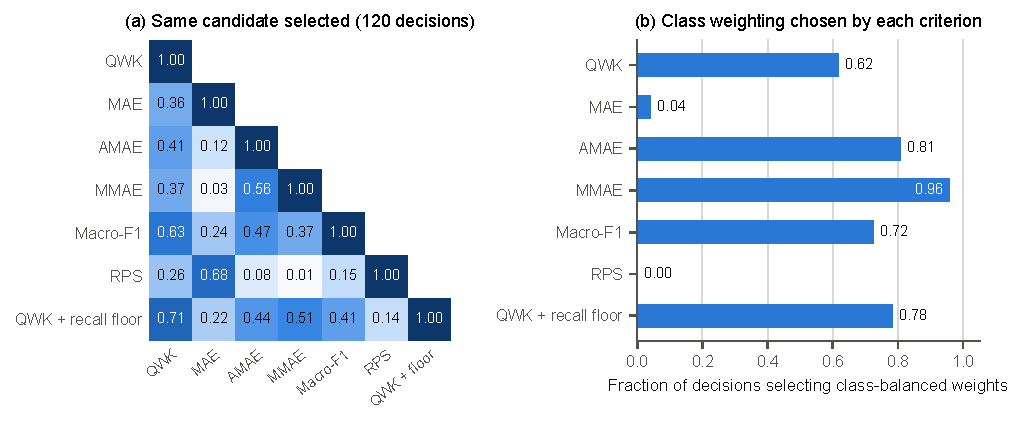
\includegraphics[width=\textwidth]{fig3_agreement_weighting.pdf}
\caption{(a) Fraction of the \NDecisions{} paired selection decisions (six primary tasks, two model families, two repeats, three outer folds) in which two criteria selected the same candidate. (b) Fraction of decisions in which each criterion selected the class-balanced version of a candidate.}\label{fig:agree}
\end{figure}

\subsection{No criterion is safe across metrics}\label{sec:res-regret}

Figure~\ref{fig:regret} shows the normalized regret of each criterion on each evaluation metric. On its own metric every criterion was close to the best single candidate (diagonal regret at most \RegOwnMax{}), but each paid elsewhere. The criteria favoured by aggregate error had the largest endpoint regret (MAE \RegEndMae{}, RPS \RegEndRps{}), and those favoured by endpoint performance paid on MAE and RPS (MMAE \RegMaeMmae{} on MAE, \QWKF{} \RegMaeCon{}). QWK and macro-F1 had low regret on each other's metric but endpoint regret of \RegEndQwk{} and \RegEndMfone{}, about halfway between the best and the worst candidate. MMAE (\RegEndMmae{}) and \QWKF{} (\RegEndCon{}) had the lowest endpoint regret.

The Friedman ranks across the 12 cells (Supplementary Table~S5) confirm the pattern. For endpoint recall the criteria differed ($\chi^2_6=\FriedEndChi$, $p\FriedEndP$): MMAE (mean rank \RankEndMmae{}) and \QWKF{} (\RankEndCon{}) ranked best, QWK, AMAE and macro-F1 lay in the middle (\RankEndQwk{}, \RankEndAmae{} and \RankEndMfone{}), and MAE (\RankEndMae{}) and RPS (\RankEndRps{}) ranked worst. The Nemenyi critical difference was \NemenyiCD{}, so only the separation of MMAE and \QWKF{} from MAE and RPS exceeds it. For QWK itself the ordering was reversed in part ($\chi^2_6=\FriedQwkChi$, $p\FriedQwkP$; QWK rank \RankQwkQwk{}, MMAE \RankQwkMmae{}).

\begin{figure}[t]
\centering
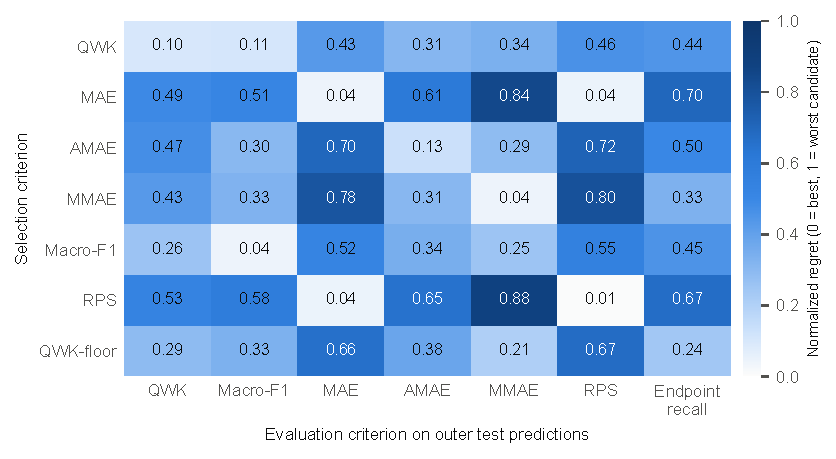
\includegraphics[width=0.85\textwidth]{fig2_regret_matrix.pdf}
\caption{Normalized cross-criterion regret on outer test predictions, averaged over the 12 primary task--family cells and two repeats. Rows: criterion used for selection; columns: metric used for evaluation. 0 corresponds to the best and 1 to the worst of the four candidates in the family, identified retrospectively.}\label{fig:regret}
\end{figure}

\subsection{Endpoint recall: what changes relative to QWK}\label{sec:res-endpoint}

Table~\ref{tab:endpoint} and Fig.~\ref{fig:endpoint} report the endpoint contrasts. Under QWK selection, several cells had low or zero endpoint recall, notably in the wine tasks, where the QWK-selected models almost never predicted the extreme scores (for PO, QWK selected the unweighted candidates in every decision). The AMAE$-$QWK difference ranged from \AmaeMin{} (MovieLens-100k, PO) to \AmaeMax{} (red wine, PO) and changed sign across tasks; over source families it was positive in \WilPosAmae{} and negative in \WilNegAmae{} blocks (Table~\ref{tab:inference}; median \WilMedAmae{}, $p=\WilPAmae$). Macro-F1 rarely differed from QWK. \QWKF{} never reduced $R_{\mathrm{end}}$: it increased it in \WilPosCon{} of the ten blocks and left the others unchanged (median \WilMedCon{}, mean \WilMeanCon{}; pooled exact $p=\WilPCon$, Holm-adjusted $p=\HolmCon$), while QWK was lower in \QwkCostNegCon{} blocks and never higher (median \QwkCostMedCon{}). In the wine tasks the floor was often infeasible on the inner predictions; all \ConFallbacks{} fallbacks to AMAE (of the \NDecisions{} \QWKF{} decisions) occurred there. MMAE behaved similarly to \QWKF{} (\WilPosMmae{} increases, \WilNegMmae{} decrease; $p=\WilPMmae$), while MAE and RPS reduced endpoint recall relative to QWK in \WilNegMae{} and \WilNegRps{} blocks, respectively. With five source families per model family, none of the per-family tests can reach $p<0.05$ (the smallest attainable two-sided exact $p$ with five blocks is 0.0625); the cross-task statistics are therefore descriptive.

\begin{table}[t]
\caption{Endpoint recall under QWK selection ($R_0$, $R_{K-1}$) and differences in mean endpoint recall $R_{\mathrm{end}}$ relative to QWK selection, with 95\% paired group-bootstrap intervals conditional on the fitted models. Last column: change in QWK caused by the recall floor. PO: proportional odds; RF: random forest.}\label{tab:endpoint}
\centering\footnotesize
\begin{tabular}{@{}llcccccc@{}}
\toprule
& & \multicolumn{2}{c}{QWK selection} & \multicolumn{3}{c}{$\Delta R_{\mathrm{end}}$ relative to QWK} & $\Delta$QWK\\
\cmidrule(lr){3-4}\cmidrule(lr){5-7}
Task & Family & $R_0$ & $R_{K-1}$ & AMAE & MMAE & \QWKF{} & \QWKF{}\\
\midrule
Wine (red) & PO & 0.00 & 0.00 & \ensuremath{+}0.53 [\ensuremath{+}0.33, \ensuremath{+}0.73] & \ensuremath{+}0.53 [\ensuremath{+}0.33, \ensuremath{+}0.73] & \ensuremath{+}0.53 [\ensuremath{+}0.33, \ensuremath{+}0.75] & \ensuremath{-}0.031 \\
 & RF & 0.00 & 0.06 & \ensuremath{+}0.11 [\ensuremath{+}0.03, \ensuremath{+}0.20] & \ensuremath{+}0.11 [\ensuremath{+}0.03, \ensuremath{+}0.21] & \ensuremath{+}0.11 [\ensuremath{+}0.03, \ensuremath{+}0.20] & \ensuremath{-}0.056 \\
Wine (white) & PO & 0.00 & 0.00 & \ensuremath{+}0.10 [\ensuremath{+}0.01, \ensuremath{+}0.23] & \ensuremath{+}0.04 [0.00, \ensuremath{+}0.08] & \ensuremath{+}0.39 [\ensuremath{+}0.22, \ensuremath{+}0.58] & \ensuremath{-}0.032 \\
 & RF & 0.07 & 0.00 & 0.00 [0.00, 0.00] & \ensuremath{+}0.06 [0.00, \ensuremath{+}0.18] & 0.00 [0.00, 0.00] & 0.000 \\
SkillCraft & PO & 0.56 & 0.70 & 0.00 [\ensuremath{-}0.01, 0.00] & 0.00 [0.00, 0.00] & 0.00 [0.00, 0.00] & 0.000 \\
 & RF & 0.46 & 0.14 & \ensuremath{+}0.19 [\ensuremath{+}0.13, \ensuremath{+}0.24] & 0.00 [0.00, 0.00] & \ensuremath{+}0.25 [\ensuremath{+}0.18, \ensuremath{+}0.32] & \ensuremath{-}0.023 \\
Restaurant & PO & 0.17 & 0.58 & \ensuremath{-}0.01 [\ensuremath{-}0.03, \ensuremath{+}0.01] & \ensuremath{+}0.05 [\ensuremath{+}0.01, \ensuremath{+}0.09] & \ensuremath{+}0.05 [0.00, \ensuremath{+}0.09] & \ensuremath{-}0.029 \\
 & RF & 0.13 & 0.63 & \ensuremath{-}0.01 [\ensuremath{-}0.02, \ensuremath{+}0.01] & 0.00 [\ensuremath{-}0.04, \ensuremath{+}0.05] & 0.00 [\ensuremath{-}0.04, \ensuremath{+}0.04] & \ensuremath{-}0.033 \\
Sushi & PO & 0.45 & 0.45 & 0.00 [0.00, 0.00] & 0.00 [0.00, 0.00] & 0.00 [0.00, 0.00] & 0.000 \\
 & RF & 0.33 & 0.32 & 0.00 [\ensuremath{-}0.01, 0.00] & 0.00 [\ensuremath{-}0.01, 0.00] & 0.00 [0.00, 0.00] & 0.000 \\
MovieLens-100k & PO & 0.52 & 0.40 & \ensuremath{-}0.40 [\ensuremath{-}0.43, \ensuremath{-}0.38] & 0.00 [0.00, 0.00] & 0.00 [0.00, 0.00] & 0.000 \\
 & RF & 0.26 & 0.38 & \ensuremath{-}0.09 [\ensuremath{-}0.10, \ensuremath{-}0.08] & \ensuremath{+}0.08 [\ensuremath{+}0.05, \ensuremath{+}0.11] & \ensuremath{+}0.05 [\ensuremath{+}0.03, \ensuremath{+}0.07] & \ensuremath{-}0.017 \\

\bottomrule
\end{tabular}
\end{table}

\begin{table}[t]
\caption{Cross-task summary of differences relative to QWK selection over source-family blocks (the two wine tasks averaged). $+/-$: number of blocks with a positive or negative difference in $R_{\mathrm{end}}$ (zeros omitted) for proportional odds (PO), random forest (RF) and both families pooled (ten blocks, not independent). Median, exact Wilcoxon $p$ and Holm-adjusted $p$ (three primary contrasts) refer to the pooled blocks and are descriptive. The last two columns give the sign counts and median of the QWK difference.}\label{tab:inference}
\centering\footnotesize
\begin{tabular}{@{}lcccrrrcr@{}}
\toprule
& \multicolumn{6}{c}{$\Delta R_{\mathrm{end}}$} & \multicolumn{2}{c}{$\Delta$QWK}\\
\cmidrule(lr){2-7}\cmidrule(lr){8-9}
Contrast & PO $+/-$ & RF $+/-$ & All $+/-$ & Median & $p$ & Holm $p$ & $+/-$ & Median\\
\midrule
AMAE $-$ QWK & 3/5 & 4/5 & 7/10 & \ensuremath{-}0.003 & 0.611 & 1.000 & 3/14 & \ensuremath{-}0.015 \\
Macro-F1 $-$ QWK & 5/2 & 3/5 & 8/7 & 0.000 & 0.847 & 1.000 & 2/14 & \ensuremath{-}0.003 \\
QWK+floor $-$ QWK & 3/0 & 5/0 & 8/0 & 0.000 & 0.008 & 0.023 & 2/6 & 0.000 \\
MMAE $-$ QWK & 6/2 & 5/3 & 11/5 & \ensuremath{+}0.002 & 0.433 & -- & 2/15 & \ensuremath{-}0.017 \\
MAE $-$ QWK & 1/6 & 2/5 & 3/11 & \ensuremath{-}0.017 & 0.035 & -- & 3/13 & \ensuremath{-}0.017 \\
RPS $-$ QWK & 1/7 & 3/5 & 4/12 & \ensuremath{-}0.028 & 0.044 & -- & 4/13 & \ensuremath{-}0.020 \\

\bottomrule
\end{tabular}
\end{table}

\begin{figure}[t]
\centering
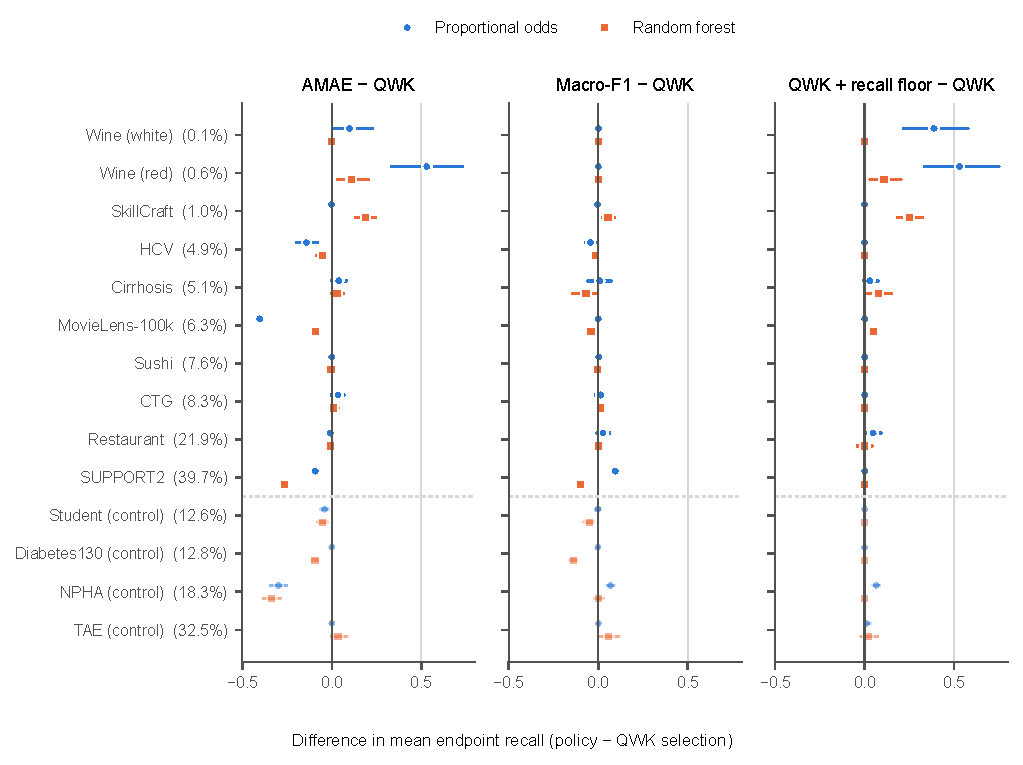
\includegraphics[width=\textwidth]{fig1_endpoint_contrasts.pdf}
\caption{Differences in mean endpoint recall between three criteria and QWK selection, with 95\% paired group-bootstrap intervals conditional on the fitted models. Tasks are ordered by the prevalence of the rarer endpoint category (in parentheses). TAE (below the dashed line) is a control task.}\label{fig:endpoint}
\end{figure}

\subsection{Why the weighting choice follows the criterion}\label{sec:res-weights}

The fixed-hyperparameter controls (Table~\ref{tab:controls}) support Remark~\ref{rem:weights}. Balanced weights increased the recall of the lower endpoint in \CtrlPosLow{} of the \CtrlN{} comparisons and mean endpoint recall in \CtrlPosEnd{} (median \CtrlMedEnd{}). They increased normalized MAE in all \CtrlPosMae{} comparisons (median \CtrlMedMae{}) but decreased normalized MMAE in \CtrlNegMmae{} (median \CtrlMedMmae{}); QWK increased in \CtrlPosQwk{} of them. A criterion built on aggregate error (MAE, RPS) therefore sees weighting as uniformly harmful, and a criterion built on the worst category (MMAE) sees it as almost uniformly beneficial, which is exactly the selection behaviour in Fig.~\ref{fig:agree}b. The upper endpoint did not always gain: in Restaurant and Sushi, where the upper endpoint is the most frequent category, weighting moved predictions away from it.

\begin{table}[t]
\caption{Fixed-hyperparameter controls: balanced minus unweighted training for the same family, hyperparameter, splits and seeds (six primary tasks $\times$ two families $\times$ two hyperparameter settings = \CtrlN{} comparisons). Counts of increases and decreases, median and range of the differences.}\label{tab:controls}
\centering\footnotesize
\begin{tabular}{@{}lrrrr@{}}
\toprule
Metric & Increase & Decrease & Median & Range\\
\midrule
Lower-endpoint recall & 23 & 0 & \ensuremath{+}0.320 & [0.000, \ensuremath{+}0.519] \\
Upper-endpoint recall & 15 & 8 & \ensuremath{+}0.121 & [\ensuremath{-}0.613, \ensuremath{+}0.700] \\
Mean endpoint recall & 21 & 3 & \ensuremath{+}0.145 & [\ensuremath{-}0.148, \ensuremath{+}0.531] \\
QWK & 17 & 7 & \ensuremath{+}0.020 & [\ensuremath{-}0.043, \ensuremath{+}0.172] \\
Normalized MAE & 24 & 0 & \ensuremath{+}0.083 & [\ensuremath{+}0.007, \ensuremath{+}0.152] \\
Normalized AMAE & 9 & 15 & \ensuremath{-}0.020 & [\ensuremath{-}0.134, \ensuremath{+}0.044] \\
Normalized MMAE & 2 & 22 & \ensuremath{-}0.204 & [\ensuremath{-}0.527, \ensuremath{+}0.071] \\
Share of endpoint predictions & 20 & 4 & \ensuremath{+}0.108 & [\ensuremath{-}0.494, \ensuremath{+}0.691] \\

\bottomrule
\end{tabular}
\end{table}

\subsection{AMAE and the constant-prediction level}\label{sec:res-constant}

Table~\ref{tab:constant} compares the candidates with the no-information level $\nu_K$ of Proposition~\ref{prop:constant}. In the three rating tasks, where QWK of the selected models was only between \QwkRangeLow{} and \QwkRangeHigh{}, \emph{all eight} candidates had a higher normalized AMAE than the constant middle-category prediction (for example, MovieLens-100k: $\nu_5=\ConstNamaeMl{}$ against a best candidate value of \BestCandNamaeMl{}). Within the pool, AMAE then prefers the candidates closest to that degenerate rule. MovieLens-100k with PO is the clearest case. The QWK-selected model (balanced weights) spread its predictions widely: prediction variance \PredVarMlPoQwk{} against a label variance of \LabVarMl{}, and \EndShareMlPoQwk{} of predictions in an endpoint category against a true share of \LabEndMl{}. It reached $R_0=\LowMlPoQwk{}$ and $R_{K-1}=\HighMlPoQwk{}$. The AMAE-selected model (no weights) concentrated its predictions in the middle (variance \PredVarMlPoAmae{}, endpoint share \EndShareMlPoAmae{}), had $R_0=\LowMlPoAmae{}$ and $R_{K-1}=\HighMlPoAmae{}$, and a worse normalized MMAE (\NmmaeMlPoAmae{} against \NmmaeMlPoQwk{}), although its normalized AMAE was lower (\NamaeMlPoAmae{} against \NamaeMlPoQwk{}). In QWK terms the dispersed model had a larger observed disagreement ($O=\ObsMlPoQwk{}$ against \ObsMlPoAmae{}) but an even larger expected disagreement ($E=\ExpMlPoQwk{}$ against \ExpMlPoAmae{}), as described in Remark~\ref{rem:qwk}.

The direction reversed where the endpoints were very rare. In red wine with PO, QWK selected an unweighted model that predicted almost only middle scores (prediction variance \PredVarWrPoQwk{}, label variance \LabVarWr{}; endpoint share \EndShareWrPoQwk{}, true share \LabEndWr{}), whereas AMAE selected the balanced model (variance \PredVarWrPoAmae{}, endpoint share \EndShareWrPoAmae{}), with $R_0=\LowWrPoAmae{}$ and $R_{K-1}=\HighWrPoAmae{}$. Neither criterion has a fixed preference for concentrated or dispersed predictions; which one protects the endpoints depends on the task.

\begin{table}[t]
\caption{Normalized AMAE of the constant middle-category prediction ($\nu_K$, Proposition~\ref{prop:constant}) compared with the best candidate, the QWK-selected and the AMAE-selected models (PO / RF), the number of candidates worse than the constant rule, and QWK of the QWK-selected models (PO / RF).}\label{tab:constant}
\centering\footnotesize
\begin{tabular}{@{}lrrrcccc@{}}
\toprule
Task & $K$ & $\nu_K$ & Best cand. & QWK-sel. & AMAE-sel. & Worse than $\nu_K$ & QWK of QWK-sel.\\
\midrule
Wine (red) & 6 & 0.300 & 0.153 & 0.212 / 0.173 & 0.154 / 0.168 & 0/8 & 0.50 / 0.54 \\
Wine (white) & 7 & 0.286 & 0.193 & 0.226 / 0.193 & 0.236 / 0.193 & 0/8 & 0.40 / 0.55 \\
SkillCraft & 7 & 0.286 & 0.124 & 0.124 / 0.131 & 0.124 / 0.132 & 0/8 & 0.73 / 0.73 \\
Restaurant & 3 & 0.333 & 0.407 & 0.424 / 0.420 & 0.414 / 0.422 & 8/8 & 0.08 / 0.07 \\
Sushi & 5 & 0.300 & 0.336 & 0.377 / 0.344 & 0.377 / 0.339 & 8/8 & 0.18 / 0.16 \\
MovieLens-100k & 5 & 0.300 & 0.320 & 0.354 / 0.326 & 0.323 / 0.321 & 8/8 & 0.20 / 0.21 \\
\midrule
TAE (control) & 3 & 0.333 & 0.328 & 0.340 / 0.390 & 0.340 / 0.389 & 7/8 & 0.29 / 0.22 \\

\bottomrule
\end{tabular}
\end{table}

\subsection{Endpoint rarity (exploratory)}\label{sec:res-rarity}

Figure~\ref{fig:rarity} relates the AMAE$-$QWK difference to the prevalence of the rarer endpoint category. Clearly positive differences occurred only in tasks whose rarer endpoint had a prevalence of about 1\% or less (both wines and SkillCraft), clearly negative ones only in MovieLens-100k (6.3\%), and all other cells showed differences close to zero (Spearman $\rho=\ModRho{}$ over \ModCells{} cells, uncorrected $p=\ModP{}$). This pattern was noticed after the results were available, the cells are not independent and three of them come from one source family; it is a hypothesis for prospective testing, not a finding. A plausible mechanism is that AMAE gives each endpoint category the weight $1/K$, which is far above its share of the data when the category is very rare but close to or below it otherwise.

\begin{figure}[t]
\centering
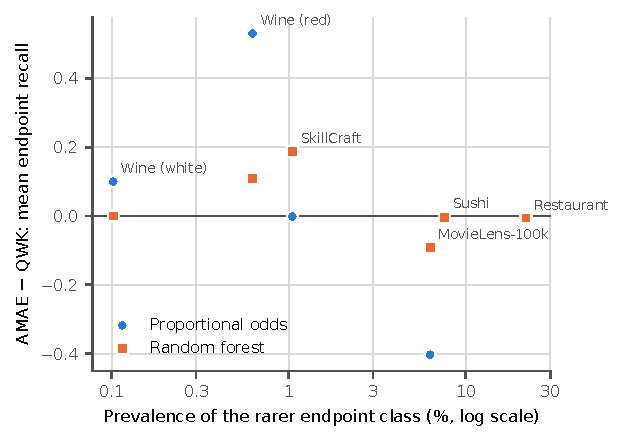
\includegraphics[width=0.62\textwidth]{fig4_endpoint_rarity.pdf}
\caption{AMAE$-$QWK difference in mean endpoint recall against the prevalence of the rarer endpoint category (log scale), for the 12 primary task--family cells. Exploratory, post hoc analysis.}\label{fig:rarity}
\end{figure}

\subsection{Controlled simulation}\label{sec:res-sim}

Under the latent Gaussian model the AMAE$-$QWK differences in $R_{\mathrm{end}}$ were small: \SimAmaeAbsSmall{} of the \SimCells{} prior--signal--family cells had an absolute difference below 0.02, and the range was \SimAmaeMin{} to \SimAmaeMax{} (Supplementary Table~S4). The largest effects occurred for random forests with rare endpoints, with opposite signs at low and high signal. The simulation therefore does not reproduce the large real-data contrasts. This is consistent with the view that these contrasts arise when weak signal, very rare endpoints and misspecified candidate models occur together, rather than from the criteria alone, but the simulation was not designed to establish such a mechanism.

\subsection{Control and superseded tasks}

In the TAE control task, whose three categories are nearly balanced, the criteria differed little and no criterion reduced endpoint recall relative to QWK (Fig.~\ref{fig:endpoint}). In the superseded eight-league SkillCraft task, AMAE selection with RF raised endpoint recall relative to QWK, in the same direction as the seven-league task but with a smaller effect (Supplementary Table~S2).

%% =====================================================================
\section{Discussion}\label{sec:discussion}

\subsection{Practical implications}

Three recommendations follow from the results. First, the selection criterion should be chosen together with, and reported alongside, the class-weighting decision, because the criterion largely determines that decision: aggregate-error criteria reject weighting and worst-class criteria adopt it. Reporting that a model was ``tuned for QWK'' without the resulting endpoint recalls hides a choice that can change endpoint recall by tens of percentage points. Second, if the endpoint categories matter, they should be protected explicitly. In our data MMAE and a simple recall floor did so most consistently, at a typical QWK cost of about 0.02. AMAE did not: its effect relative to QWK changed sign. Third, AMAE should be read against its no-information level $\nu_K=(K+1)/(4K)$ (odd $K$). Values near $\nu_K$ are compatible with a constant middle-category rule that never predicts an endpoint. In low-signal tasks, minimizing AMAE can favour candidates that drift towards that rule.

These findings complement the binary-classification study of \citet{delaCruzHuayanay2024}, in which some metrics consistently selected good models under simulation. In the ordinal setting studied here, no single criterion was close to optimal on all metrics, and the choice is a trade-off that should be made explicit. Relative to earlier ordinal work that tuned models with different metrics \citep{Binotto2025}, our results add the class-weighting dimension, the endpoint focus and the constant-prediction reference for AMAE. Selecting on pooled inner predictions and evaluating on untouched outer folds avoids the optimistic bias of selecting and evaluating on the same data \citep{Varma2006,Cawley2010}. The regret analysis, which looks at the test data, is reported only descriptively.

\subsection{Limitations}

The evidence is limited in several respects. There are six primary tasks from five source families, three of which are low-signal rating tasks with a shared item pool, and two wine tasks with very few endpoint cases. The candidate pool is deliberately small: two families, two hyperparameter settings each and two weighting options. Larger pools may reduce or amplify the differences. All criteria use argmax decoding; criterion-specific decoding rules \citep{Delgado2026} were not studied. Two repeats of three-fold cross-validation and group bootstrap intervals conditional on fitted models do not capture all sources of uncertainty, and the cross-task tests have low power. The study proceeded in two stages, with locally frozen but not externally registered protocols. SkillCraft relies on the source's one-replay-per-participant design, and the endpoint-rarity pattern is post hoc. A prospective study on additional tasks with pre-specified hypotheses is needed before these patterns can be generalized.

%% =====================================================================
\section{Conclusion}\label{sec:conclusion}

In tabular ordinal classification, the criterion used for model selection is not a neutral detail. Within one fixed candidate pool, it determined whether class weighting was used, it changed the selected model in most paired decisions, and it changed endpoint recall by up to about 0.5 in either direction relative to QWK. No criterion was safe on all metrics. Worst-class or recall-constrained criteria protected the endpoint categories at a small QWK cost, AMAE did not reliably do so, and AMAE values should be compared with the constant-prediction level $(K+1)/(4K)$. Reporting endpoint recall and worst-class error together with the selection criterion is a simple step that makes these trade-offs visible.

%% =====================================================================
\backmatter

\bmhead{Supplementary information}
The online Supplementary Information contains full per-policy metrics for all tasks (Table~S1), all policy contrasts with bootstrap intervals (Table~S2), all fixed-hyperparameter controls (Table~S3), the simulation results (Table~S4), Friedman ranks for all evaluation metrics (Table~S5), and data provenance and feature definitions.

%% AUTHORS: complete or confirm every statement below.
\section*{Statements and Declarations}

\bmhead{Funding} [To be completed by the authors, e.g.\ ``The authors did not receive support from any organization for the submitted work.'']

\bmhead{Competing interests} [To be confirmed by the authors, e.g.\ ``The authors have no relevant financial or non-financial interests to disclose.'']

\bmhead{Ethics approval and consent to participate} This study is a secondary analysis of publicly documented, de-identified data sets; no new data were collected from human participants. [Authors: confirm with your institution whether a formal statement or exemption is required.]

\bmhead{Data availability} The wine, SkillCraft, Restaurant and TAE data are available from the UCI Machine Learning Repository under CC BY 4.0 (DOIs in the reference list). The Sushi and MovieLens-100k data permit research use but not redistribution and must be obtained from their providers \citep{Kamishima2003,Harper2015}. Scripts that reproduce the task definitions, user selection and splits from the original files are provided with the code. Aggregate results (all tables and figures) are included in the Supplementary Information.

\bmhead{Code availability} [Authors: insert the repository URL or ``available from the corresponding author on reasonable request''. The proportional-odds implementation is taken from the authors' earlier code base; confirm the licence before public release.]

\bmhead{Author contributions} [To be completed by the authors.]

\bibliography{refs}

\end{document}
